\documentclass[preprint]{aastex}

\bibliographystyle{apj}

%COMPILE WITH LaTeX->PS. FIGURES ARE EPS

\def \teff {T_{\rm eff}}

\def \phir {\Phi_{\rm R}}

\def \fov {24$^{\circ}$ }
\def \aeff {69.1 cm$^2$ }

\begin{document}

\title{Simulating the Planet Yield of the Transiting Exoplanet Survey Satellite}

\author{Peter W. Sullivan, Courtney D. Dressing, Josua N. Winn, Alan M. Levine, Roland K. Vanderspek, George R. Ricker}
%\altaffiltext{1}{MIT-Kavli Institute for Astrophysics and Space Research}

%\begin{abstract}

%\end{abstract}

\section{Introduction}
\subsection{Stellar population}
What is the radius function of the local solar neighborhood? (plot of $\phir$)
\subsection{Planet population}
Kepler results and the number of expected (transiting) planets in the nearest $\sim$100 pc. Should we include Petigura rates or Dressing-Charbonneau rates?

\section{Description of TESS}
\subsection{Mission and survey}

\begin{figure}[hbtp]
\begin{center}
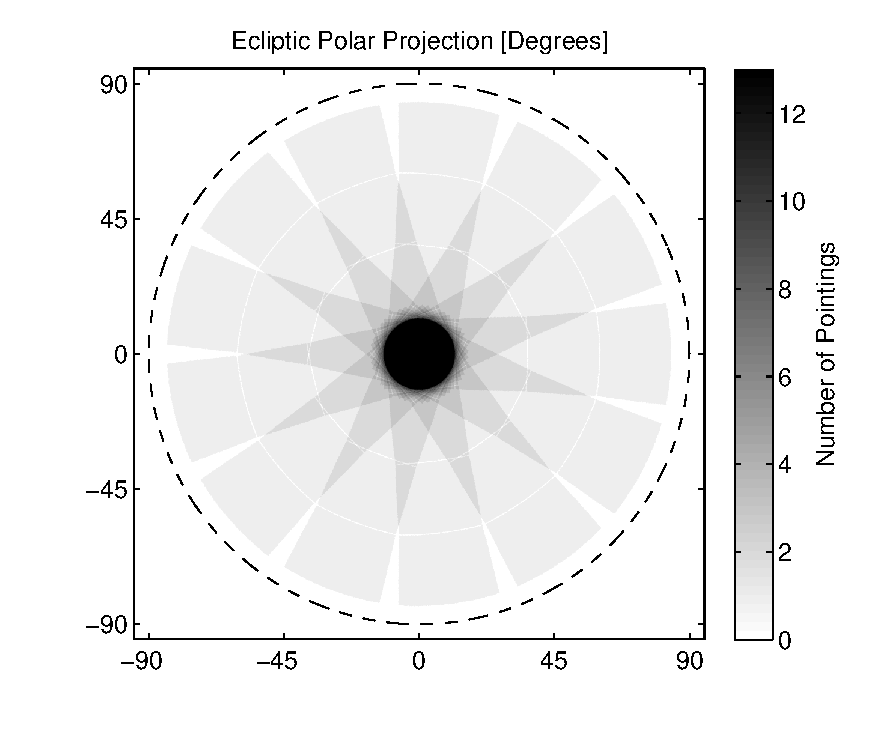
\includegraphics[width=0.5\textwidth]{npnt.eps}
\caption{The number of 26.7-day pointings TESS spends on a given star is a function of its ecliptic coordinates. Here, the number of pointings are shown in a polar ecliptic projection; the pointings in the northern and southern ecliptic hemispheres are symmetric. Coverage near the ecliptic (dashed line) is sacrificed in favor of coverage near the ecliptic poles, which receive continuous coverage for 360 days.}
\end{center}
\end{figure}

\subsection{Optics and CCD}
FOV, EPD, PSF, bandpass, noise. \\
Can we say ``as we will present at PDR"? \\
Counts vs. spectral type

\section{Simulations}
\subsection{Star Catalog}
How we select from $\phir$
\subsection{Planet Population}

\begin{figure}[hbtp]
\begin{center}
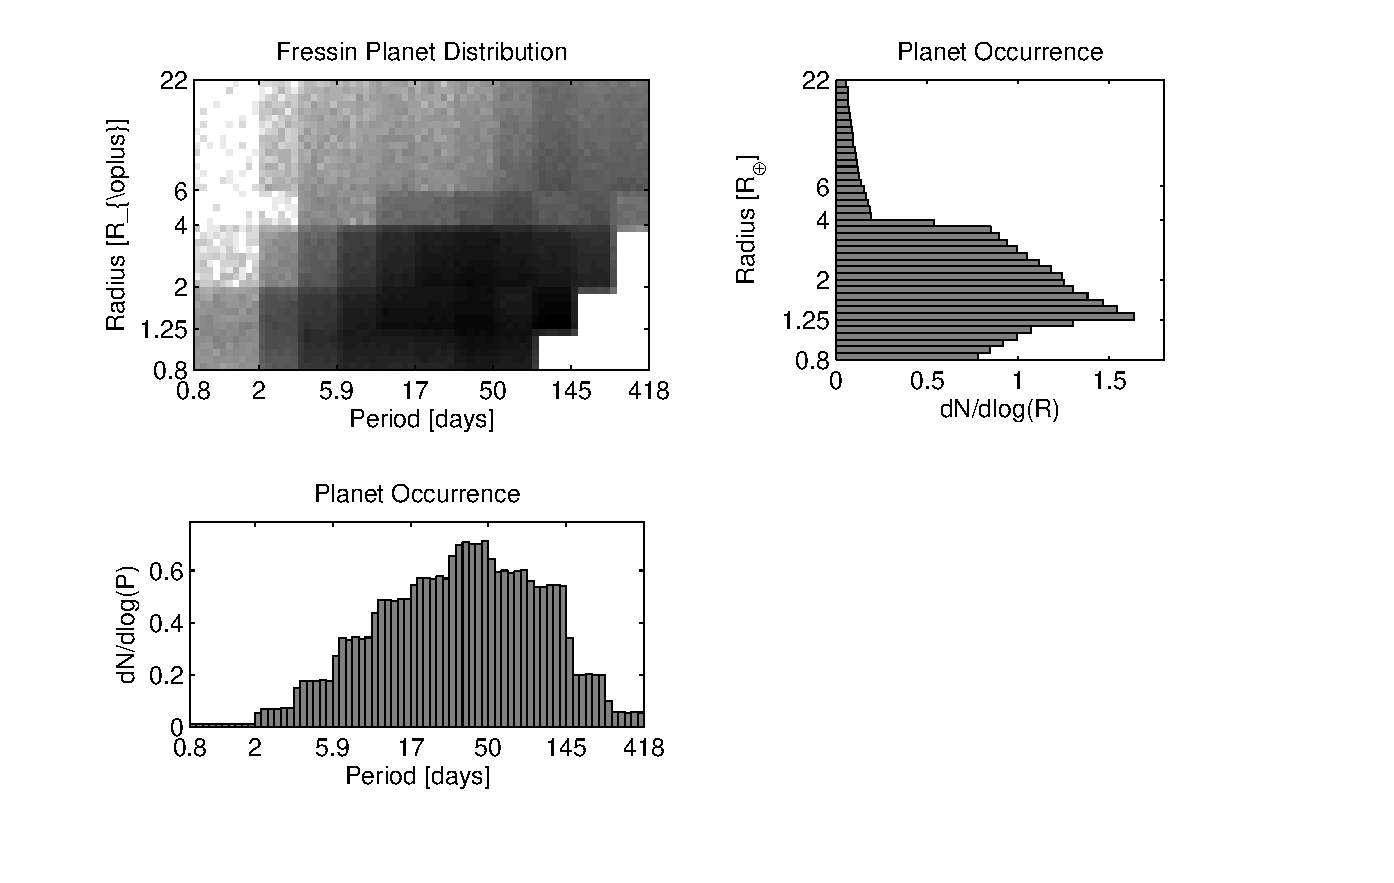
\includegraphics[width=0.7\textwidth]{fress.eps}
\caption{We adopt the planet occurrence rates as a function of radius and period from \citet{fressin2013}, which are calculated from the \textit{Kepler} mission. Within the coarse bins in the radius-period plane (\textit{upper left panel}), we assume the periods are distributed according to $P^{-1}$, giving a flat distributions in $\log{P}$ (\textit{lower left panel}). For planet radii $R_p>1.25R_{\oplus}$, we assume the radii are distributed by $R_p^{-1.7}$, and for $R_p<1.25R_{\oplus}$, we assume a flat distribution in $R_p$. This gives a fairly smooth distribution in $R_p$ (\textit{upper right panel}).}
\end{center}
\end{figure}

\subsection{Background Model}
\subsection{Zodiacal Light}
HST spectrum
\subsection{Background Stars}
Besan\c{c}on model
\subsection{Noise model}
Read noise, optimal apertures
\subsection{Detection criteria}
Observed number of transits
Detection thresholds (7$\sigma$)

\begin{figure}[hbtp]
\begin{center}
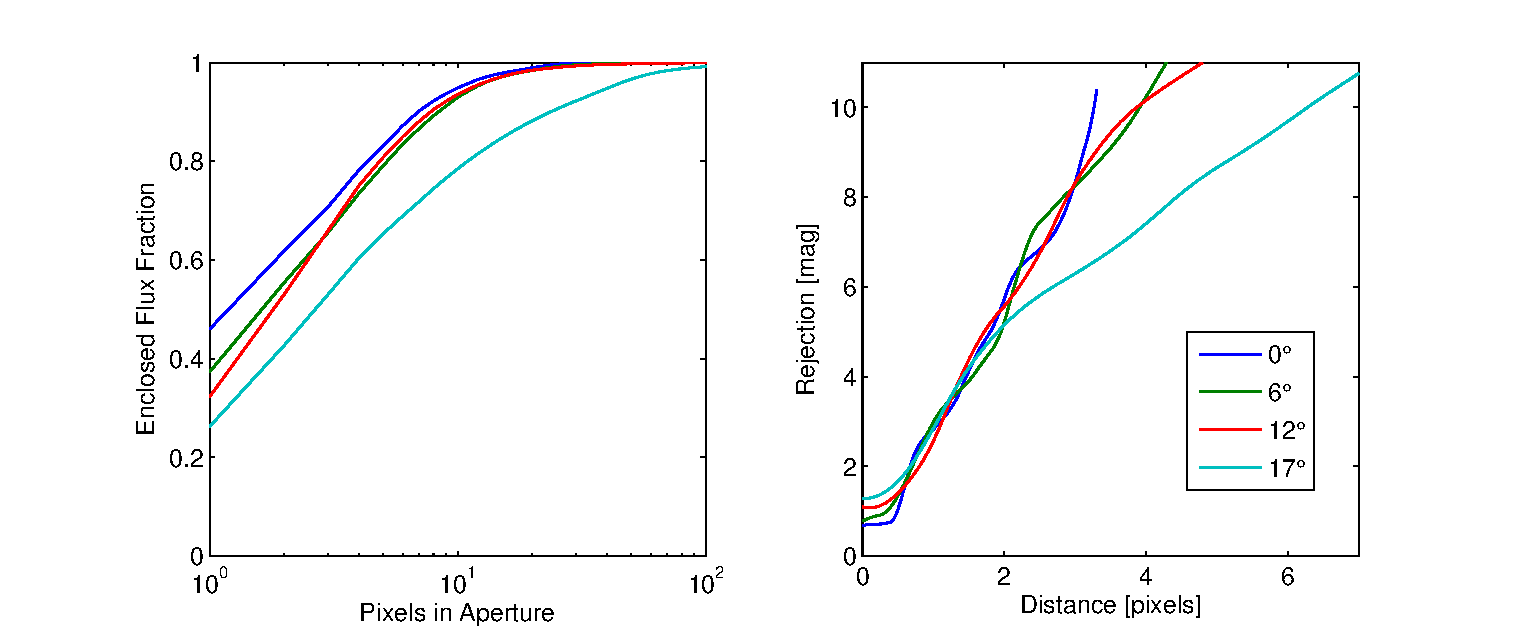
\includegraphics[width=0.9\textwidth]{npix.eps}
\caption{The TESS optics serve two purposes: to focus the light from a target star into as few pixels as possible and to reject the light from nearby stars as much as possible. On the left, we plot the fraction of accumulated flux over the number of pixels in the photometric aperture. On the right, we plot the point source rejection ratio (PSRR), expressed as a difference in astronomical magnitudes, over the distance between a target pixel and a contaminating star.}
\end{center}
\end{figure}

\section{Results}
\subsection{Planet Yields}
\subsection{Habitability of the TESS-detected planets}
Plot of $S$ vs. $\teff$ for detected planets
\subsection{Observations of the Kepler Objects of Interest}
Histogram of transit timing precision.

\section{Follow-up of the TESS detections}
\subsection{Photometry}
Plot of transits in ppm/hr versus ($I_C$ and/or $J$) magnitude.
\subsection{Radial Velocity}
Plot of RV $K$ vs. ($I_C$ and/or $V$) magnitude.

%\begin{figure}
%\epsscale{1.0}
%\plotone{filters.eps} 
%\caption{\emph{Left:} Intermediate- and narrow-band filters used to detect LAEs. \emph{Right:} Filters used to detect the Ly-$\alpha$ absorbers. For reference, the composite LBG spectrum from \citet{shap03} is also plotted near the expected redshifts of the LAEs and background galaxies.}
%\label{filter}
%\end{figure}

%\section{Conclusions}

\acknowledgements

\clearpage

\begin{thebibliography}{}

\bibitem[Binney \& Merrifield(1998)]{1998gaas.book.....B} Binney, J.,
  \& Merrifield, M.\ 1998, Galactic astronomy (Princeton University
  Press)

\bibitem[Bochanski et al.(2010)]{2010AJ....139.2679B} Bochanski,
  J.~J., Hawley, S.~L., Covey, K.~R., et al.\ 2010, \aj, 139, 2679

%\bibitem[Boyajian et al.(2012)]{2012ApJ...757..112B} Boyajian, T.~S.,
%  von Braun, K., van Belle, G., et al.\ 2012, \apj, 757, 112

\bibitem[Covey et al.(2008)]{2008AJ....136.1778C} Covey, K.~R.,
  Hawley, S.~L., Bochanski, J.~J., et al.\ 2008, \aj, 136, 1778

\bibitem[Cruz et al.(2007)]{2007AJ....133..439C} Cruz, K.~L., Reid,
  I.~N., Kirkpatrick, J.~D., et al.\ 2007, \aj, 133, 439
  
\bibitem[Fressin et al.(2013)]{fressin2013} Fressin, F., Torres, 
G., Charbonneau, D., et al.\ 2013, \apj, 766, 81 

\bibitem[Reid et al.(2002)]{2002AJ....124.2721R} Reid, I.~N., Gizis,
  J.~E., \& Hawley, S.~L.\ 2002, \aj, 124, 2721

\bibitem[Reid \& Hawley(2005)]{2005nlds.book.....R} Reid, I.~N., \&
  Hawley, S.~L.\ 2005, New Light on Dark Stars: Red Dwarfs, Low-Mass
  Stars, Brown Dwarfs (Springer-Praxis)

\bibitem[Zheng et al.(2001)]{2001ApJ...555..393Z} Zheng, Z., Flynn,
  C., Gould, A., Bahcall, J.~N., \& Salim, S.\ 2001, \apj, 555, 393

\bibitem[Zheng et al.(2004)]{2004ApJ...601..500Z} Zheng, Z., Flynn,
  C., Gould, A., Bahcall, J.~N., \& Salim, S.\ 2004, \apj, 601, 500

\end{thebibliography}

\end{document}
